\section{Method}
\label{sec:method}

We frame stagnation detection as window-level binary classification over agent trajectories.
Silver labels are generated via weak supervision from three labeling functions, then used to train and evaluate three detection approaches: structural features, a neural embedding probe, and an LLM-as-judge baseline.
Figure~\ref{fig:pipeline} provides a system overview.

\begin{figure*}[t]
\centering
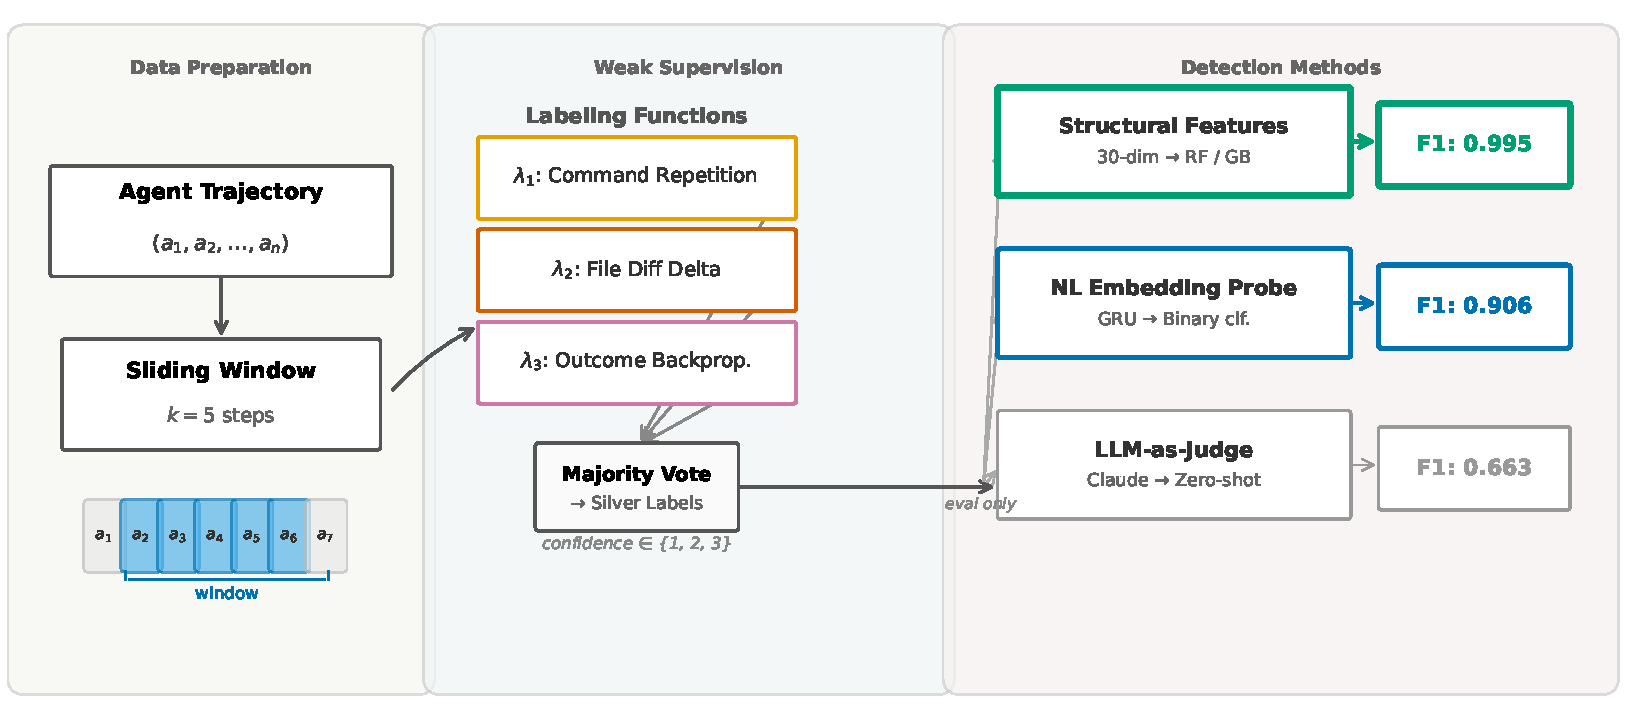
\includegraphics[width=\textwidth]{../../figures/paper/fig_pipeline.pdf}
\caption{System overview. (Left) Agent trajectories are segmented into overlapping windows of $k{=}5$ steps. (Center) Three labeling functions vote on each window; majority vote produces silver labels with confidence 1--3. (Right) Three detection approaches compared: structural features (30-dim), NL embedding probe (GRU), and LLM-as-judge (eval only, not trained on silver labels).}
\label{fig:pipeline}
\end{figure*}

%-------------------------------------------------------------------
\subsection{Problem Formulation}
\label{sec:problem}

Given an agent trajectory $T = (a_1, a_2, \ldots, a_n)$ where each $a_t$ is an action (e.g., a shell command, file edit, or API call), we partition it into overlapping sliding windows $w_i = (a_i, \ldots, a_{i+k-1})$ with window size $k{=}5$ and stride 1.
The task is to assign each window a binary label $y_i \in \{0, 1\}$, where 0 denotes \emph{stagnation} (the agent is stuck or unproductive) and 1 denotes \emph{progress} (the agent is making meaningful headway toward the task goal).

The window formulation offers two advantages over alternatives.
Compared to step-level scoring, windows capture short-range temporal patterns---such as a sequence of repeated failed attempts---that individual actions cannot express.
Compared to trajectory-level labeling, windows provide the granularity needed to pinpoint \emph{when} stagnation begins and ends within a single task attempt, enabling downstream interventions such as early termination or strategy switching.

%-------------------------------------------------------------------
\subsection{Weak Supervision Pipeline}
\label{sec:weak_supervision}

Prior gold-standard annotations for agent stagnation at the window level are unavailable; we construct a stratified gold set (\S\ref{sec:gold_set}).
Manual annotation is expensive: each window requires reviewing $k$ actions with full context (command text, outputs, file diffs), taking an estimated 2--3 minutes per window.
We therefore adopt a data programming approach \citep{ratner2016dataprogramming,ratner2019snorkel}: multiple labeling functions (LFs) provide noisy votes that are aggregated into silver labels.
Each LF $\lambda_j : w_i \to \{0, 1, \bot\}$ examines a window and emits a vote: stagnation (0), progress (1), or abstain ($\bot$).

\subsubsection{Labeling Functions}
\label{sec:labeling_functions}

We design three LFs that target complementary signals of stagnation.

\paragraph{Command repetition ($\lambda_1$).}
Computes the proportion of repeated commands within $w_i$; a high ratio triggers a stagnation vote.
Never abstains.
Fires on 65.5\% of SWE-Agent windows but only 5.4\% of OH windows (97.9\% precision), reflecting agent-specific temporal dynamics (\S\ref{sec:cmd_rep_ablation}).

\paragraph{File diff delta ($\lambda_2$).}
Measures the fraction of steps producing code modifications.
Low modification frequency triggers stagnation; ${>}1$ edited file triggers progress; otherwise abstains.
On OH, achieves 87.5\% recall (99.9\% precision), the most reliable cross-coding-agent signal.

\paragraph{Outcome backpropagation ($\lambda_3$).}
Uses the final task outcome as distant supervision: unresolved tasks' last windows receive stagnation votes; resolved tasks receive progress votes; all others abstain.
Unlike $\lambda_1$/$\lambda_2$, $\lambda_3$ propagates a global signal backward through time.


\subsubsection{Label Aggregation}
\label{sec:label_aggregation}

Silver labels are produced by majority vote among non-abstaining LFs:
\begin{equation}
y_i = \text{MV}\bigl(\{\lambda_j(w_i) : \lambda_j(w_i) \neq \bot\}\bigr)
\label{eq:mv}
\end{equation}
We define the confidence of each label as the number of non-abstaining LFs that agree with the winning label: $\text{conf}_i = |\{j : \lambda_j(w_i) \neq \bot \;\text{and}\; \lambda_j(w_i) = y_i\}| \in \{1, 2, 3\}$.
Conf${=}1$ arises when a single non-abstaining LF determines the label---either because only one LF votes or because two LFs disagree with no clear majority---producing the most ambiguous labels.
The conf${\geq}$2 subset, where at least two non-abstaining LFs agree on the winning label, serves as the primary evaluation set throughout this work.
This stratification allows us to separately analyze model behavior on high-confidence vs.\ ambiguous windows (\S\ref{sec:main_results}).

%-------------------------------------------------------------------
\subsection{Detection Methods}
\label{sec:detection_methods}

\subsubsection{Structural Features}
\label{sec:structural_features}

We extract a 30-dimensional feature vector from each window, requiring no pretrained model or GPU.
Features span four categories:
(1)~\emph{repetition}: exact command repeat ratio, fuzzy match ratio (Levenshtein-based), and unique command ratio;
(2)~\emph{file operations}: counts of file creates, modifications, and deletions within the window;
(3)~\emph{edit patterns}: edit distances between consecutive actions, capturing how much the agent's behavior changes step-to-step;
(4)~\emph{output statistics}: entropy of command outputs and action type distribution features.
These features are fed to three classifiers: Logistic Regression (LR), Random Forest (RF), and Gradient Boosting (GB).
Because several structural features overlap with the signals used by the labeling functions (e.g., repetition ratios relate to $\lambda_1$), structural classifiers can partially reconstruct the LF voting process.
We discuss this circularity and its implications in \S\ref{sec:main_results}.

\subsubsection{NL Embedding Probe (ProgressProbe)}
\label{sec:progressprobe}

Each action $a_t$ is encoded as a natural language description and embedded using Qwen3-Embedding-0.6B \citep{zhang2025qwen3embedding} into a 1024-dimensional vector.
The $k$ embeddings within a window form a sequence that is processed by a 2-layer GRU \citep{cho2014gru} with hidden size 256 and dropout 0.1.
An attention mechanism \citep{bahdanau2015attention} computes a weighted combination of the GRU hidden states, yielding a single window-level representation.
This representation is passed through a fully connected layer with sigmoid activation for binary classification.
Training uses binary cross-entropy loss with early stopping (patience 5) on a validation set.

The GRU architecture is motivated by the sequential nature of actions within a window: the order in which commands are issued (e.g., repeated failures followed by a different approach) carries diagnostic information that bag-of-embeddings methods discard.
We also evaluate two simpler embedding baselines to isolate the contribution of temporal modeling: (1)~mean-pooled Qwen3 embeddings with logistic regression, and (2)~cosine similarity between consecutive window embeddings with a validation-tuned threshold.

\subsubsection{LLM-as-Judge Baseline}
\label{sec:llm_judge}

We prompt Claude Sonnet 4.6 in zero-shot mode to classify each window as stagnation or progress, given the textual descriptions of actions within the window.\footnote{Extended LLM evaluation including chain-of-thought prompting, few-shot examples, and multi-model comparison is reported in Appendix~\ref{sec:llm_extended}.}
The LLM judge establishes a cost-performance reference: at \$11.66 per test set, its zero-shot F1 of 0.663 demonstrates that stagnation detection is non-trivial even for capable LLMs without task-specific adaptation.
This baseline is not used in the silver label pipeline.

%-------------------------------------------------------------------
\subsection{Temporal Label Models}
\label{sec:temporal_models}

The three LFs occupy distinct temporal niches relative to stagnation onset (\S\ref{sec:lf_temporal}): $\lambda_1$ leads by ${\sim}2$ steps, $\lambda_2$ is near-concurrent, and $\lambda_3$ lags by ${\sim}7$ steps.
This motivates testing whether temporal aggregation improves over majority vote.
We evaluate three temporal label models---Time-Varying Weights (TWV) with Gaussian kernel smoothing, a Hidden Markov Model (HMM) \citep{safranchik2020linkedhmm} over joint LF patterns, and a Lag-Aware HMM that models each LF's temporal offset---alongside two generative i.i.d.\ models: FlyingSquid \citep{fu2020flyingsquid} and Snorkel MeTaL \citep{ratner2019snorkelmetal}---all descendants of classical EM-based annotator models \citep{dawid1979em}.
Full model specifications appear in Appendix~\ref{sec:app_temporal_models}.